\documentclass[a4paper,11pt]{report}
\usepackage[T1]{fontenc}
\usepackage[utf8]{inputenc}
\usepackage{lmodern}
\usepackage[francais]{babel}
\usepackage{graphicx}
\usepackage{array}

\title{Data wars}
\author{Guillaume LAROYENNE, Nathan PRETOT,\\ Jeremy RENAUD,Tom SALVI, Pierre VALENZA}

\begin{document}

\maketitle
\tableofcontents

\begin{abstract}
\end{abstract}

\chapter{Mise en œuvre}
  \section{Logiciel et méthode utilisé}
  \subsection{Organisation du projet}
     \begin{description}
       \item[Logiciel de gestion de versions :] nous avons utilisé \textit{git} et la plateforme \textit{GitHub} pour gérer le partage des fichiers et la gestion des versions. Nous avons utilisé ceci car, l'ayant appris en cours, tout les membres du projet étaient capable de l'utiliser.
       \item[Communication :] pour la communication d'information importante et d'information durable, l'utilisation de mail ou encore de système de discussion instantanée tel que \textit{messenger}. En plus de tout ceci, l'utilisation du logiciel de discussion \textit{Discord} nous a permit de parler du projet de vive voix.
       \item[Répartition des tâches :] pour la répartition des tâches et l'organisation du projet, nous nous sommes servis du site \textit{Trello}. Son interface simple, mais efficace, nous a permit de suivre l'avancé du projet.
     \end{description}
  
  \subsection{Jeu}
    \begin{description}
      \item[Langage de programmation :] \textit{Java} fut choisit pour plusieurs raisons, notamment, étant le langage le plus utilisés lors de notre formation, tout les membres de notre groupe avait un niveau équivalent sur celui-ci. De plus, la création d'une interface graphique en \textit{Java}, ayant été vue en cours, était donc connu par notre groupe.   
      \item[Base de données :] nous avons décidé d'utiliser \textit{MySQL}. Nous avons fait ce choix pour la simplicité d’intégration avec \textit{java} via la bibliothèque \textit{mysql-connector}.
      
    \end{description}
  
    \subsection{Interface}
    \subsubsection{Le Paradigme MVC}
    Nous avons structuré notre projet avec le paradigme MVC ( Modèle, Vue, Contrôleur), car ce format s'adapte parfaitement au jeu en tour par tour. En effets il permet de juste envoyer la partie modèle avec le réseau sans toucher ni aux contrôleurs ni à la vue.   
    \subsubsection{La bibliothèque graphique Java Swing}
    Nous avons décidé d'utiliser la bibliothèque graphique Java Swing car nous l'avions déjà utiliser sur plusieurs projets et que c'est la technologie que nous maitrisions le plus.
    \subsubsection{Logiciels}
    Voici les différents logiciels utilisés pour réaliser les graphismes.

    \begin{description}
      \item[Gimp :] Nous avons utilisé ce logiciel pour la modification des images de la vue. Nous avons choisi ce logiciel car c'est un logiciel gratuit et que l'on maitrisait déjà un peu. 
      \item[Inkscape :] Nous avons utilisé ce logiciel pour la création des images de la vue. Nous avons choisi inkscape car c'est un logiciel libre qui permet de faire du dessin vectoriel, et donc de pouvoir facilement redimensionner les images. 
    \end{description}



\subsection{Réseau}

\subsubsection{Langage utilisé}
Le langage Java est utilisé pour le serveur et le client pour sa simplicité. En effet java permet un échange des données extrêmement simple grâce à la sérialisation de ses objets. De plus la création des connexions réseau se fait rapidement.
En utilisant ce langage, la communication entre les programmes a donc pu être réalisée rapidement, permettant aux développeurs de se consacrer davantage sur les protocoles.

\subsubsection{Bibliothèque utilisée}
Les bibliothèques utilisées pour le serveur sont :
\begin{enumerate}
  \item GraphStream, pour la visualisation de l'état du serveur sous forme de graphe. Car cette librairie est très similaire à la librairie PHP que nous avons utilisée aux parts avant.
  \item MySQL Connectors, pour la communication avec la base de donné. Car cette librairie contient de nombreux outils compatibles avec Java Swing.
  \item Java Zoom, pour la lecture de fichiers audio. Car cette librairie est très simple d’utilisation et contient une bonne documentation.
\end{enumerate}

\subsubsection{Test unitaire}
Pour pouvoir identifier rapidement les erreurs éventuelles dans les protocoles, ainsi que des failles de sécurité, des tests unitaires ont été réalisés. Ces tests ont été réalisées avec la librairie JUNIT. 


	

  \section{Répartition du travail}
    Ce projet mettant en œuvre une grande diversité de domaine (site web, jeu, serveur, base de données, graphisme), nous n'avons donc pas eu d'autres choix que de répartir notre effectif sur les différents domaines. Laissant ainsi presque tout les domaines (à part modèle) couvert par une seule personne, nous laissant la disposition suivante :
    \begin{description}
      \item[Jeremy : ] implémentation des interfaces et des contrôleurs.
      \item[Tom : ] travail sur une partie du modèle du jeu.
      \item[Guillaume :] modélisation et création du serveur et des communications réseaux.
      \item[Pierre :] création du site web.
      \item[Nathan :] modélisation et création de la base de données. Modélisation du jeu et réalisation d'une partie de celui-ci.
    \end{description}
    
    \begin{figure}[th]
      \begin{center}
        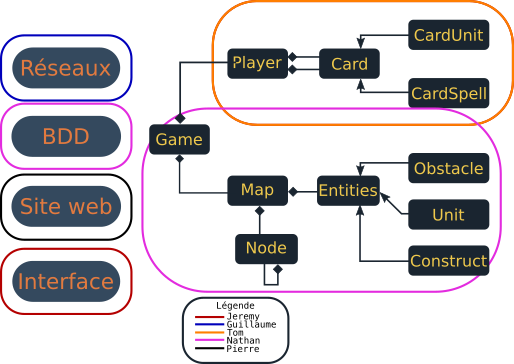
\includegraphics[scale=0.365]{Assets/UMLRepartition.png}
        \caption{Répartition du travail}
        \label{RepTravail}
      \end{center}
    \end{figure}
    
    De plus des éléments du domaine informatiques, notre projet nous a demandé la création entière d'un jeu, nous demandant une réflexion autours des règles et fonctionnalités de celui-ci, ainsi que de créer des cartes innovantes pour celui-ci. Cette partie à été endossée par l'ensemble de l'équipe.
    
  \section{Gestion du temps}
    Le projet a débuté sur la conception du jeu. C'est-à-dire la création des règles, ainsi que les éléments de modélisation au niveau informatique ( MCD, UML, etc...).  C'est étape, qui a durée un mois et demis, fut suivit du début de la phase de programmation du réseau et du jeu. La partie interface commença un peu plus tard, car elle nécessitais d'avoir une partie du modèle de terminée pour commencer. Le site web ne commença qu'a partir de janvier car celui-ci n'était pas prévus dans le travail initiale. Une première version du jeu en mono-poste fut terminée au milieu des vacances de février, suivis de près par la version réseau.
    \begin{figure}[th]
      \begin{center}
        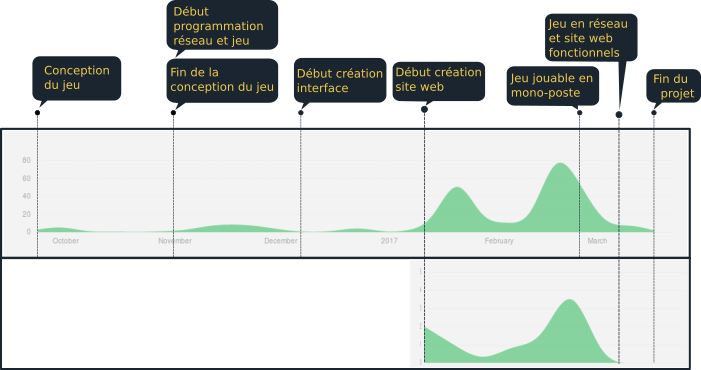
\includegraphics[scale=0.5]{Assets/gestionTemps.png}
        \caption{Gestion du temps par rapport à la courbe des \textit{commits} \textit{GitHub}}
        \label{RepTime}
      \end{center}
    \end{figure}
  

    \section{Rendu}
      \subsection{Les composants du projet}
        A ce jour, le projet comporte :

 	\subsection{Site internet}

	\paragraph{}
       Data wars est un jeu qui utilise une base de données contenant les informations des utilisateurs ainsi que les cartes qui leur sont nécessaires. Pour accéder à ces données et les modifier, nous avons mis en place un site web réalisé en PHP afin d'y apporter un niveau de sécurité suffisant lors de sa modification. L'architecture du site est réalisé en Modèle-Vue-Contrôleur (MVC) ce qui améliore la facilité de maintenance du site, d’ailleurs pour la vue nous avons fait le choix d'en faire un site \textit{responsif} afin d'y accéder depuis n'importe quel appareil. 

	\subsubsection{Partie administrateur} 
	\paragraph{}

    	\begin{figure}[th]
      	 \begin{center}
          
\includegraphics[scale=0.25]{Assets/navbar_admin.png}
          \caption{Barre de navigation côté administrateur}
          \label{RepTravail}
         \end{center}
        \end{figure}

	 La première du site n'est accessible que par les administrateurs afin de pouvoir mettre à jour : 
	\begin{enumerate}
		\item les cartes
		\item les joueurs
		\item les effets
	\end{enumerate}Il a donc été nécessaire d'y installer une sécurité afin que les données enregistrées soient correctes pour ainsi éviter que des conflits apparaissent. Pour cela nous utilisons un framework : Silex, qui offre donc des services pour mettre en place des contraintes qui doivent être respectées par l'utilisateur pour que les données saisies soient envoyées dans la base de données.

	\newpage

	\subsubsection{Partie joueur}
	\paragraph{}

	\begin{figure}[th]
      	 \begin{center}
          
\includegraphics[scale=0.25]{Assets/navbar_joueur.png}
          \caption{Barre de navigation côté joueur}
          \label{RepTravail}
         \end{center}
        \end{figure}

      La seconde partie du site est donc accessible par les joueurs qui d'ailleurs devront créer leur compte sur le site. À partir d'ici il est nécessaire de respecter les contraintes du jeu : 

	\begin{enumerate}
		\item la taille du deck a une limite à ne pas dépasser
		\item une carte n'est pas dans le deck ou l'est maximum une fois
	\end{enumerate}Pour cela on empêche tout simplement l'ajout lorsque cette limite est atteinte à l'aide de requêtes SQL qui compte et compare les cartes du jeu avec celles présentes dans le deck.
	
	\paragraph{}
	L'objectif principal a donc été de réaliser une vue qui soit agréable pour la construction des decks. Ainsi la modification se fait sur une seule page où le deck du joueur, les cartes du jeu, et une vue détaillée de la carte sélectionnée sont visibles. De cette manière le joueur peut donc naviguer entre les cartes de manière aisée. Toutefois lorsqu'une action est effectuée la page doit se recharger, on pourrait donc améliorer cette partie pour rendre la navigation plus fluide aux joueurs en y ajoutant du \textit{Javascript}.




      \subsubsection{Un système réseau avec interface réutilisable\\ sur d'autres projets :}

        Il permet de créer un groupe, envoyer une invitation au membres connectés, ces derniers peuvent gérer les invitations reçus ( accepter ou non ) l'invitation est limitée dans le temps pour éviter d'attendre un joueur éternellement. Une fois le groupe créé l'hôte peut lancer la partie.   


        \begin{center}
        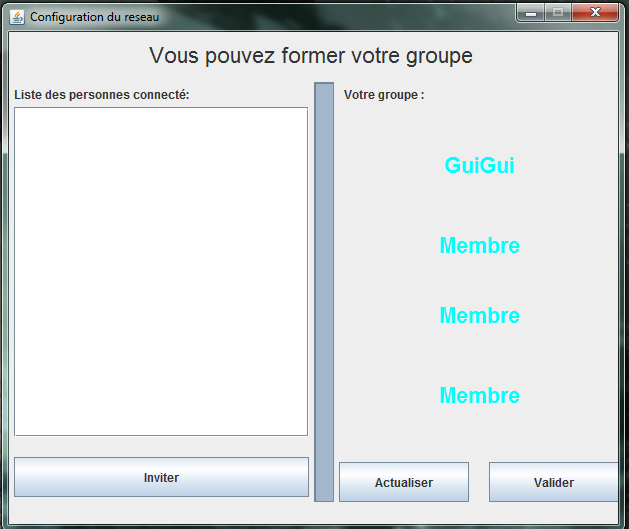
\includegraphics[scale=0.5]{Assets/connection3.png} 
        \end{center}

        \subsubsection{Un jeu jouable en Réseau de 2 à 4 joueurs.}

        Dans le jeu on peut récupérer le deck en fonction du joueur, jouer des cartes, déplacer des unités, attaquer des unités ennemies, capturer des bâtiments de ressources, voir les informations des entités sur la carte. La gestion des ressources est fonctionnelle.

         On peut attaquer le QG ennemi pour gagner la partie.

        La partie de chaque joueur est synchronisée à chaque fin de tour d'un joueur.
        \begin{center}
        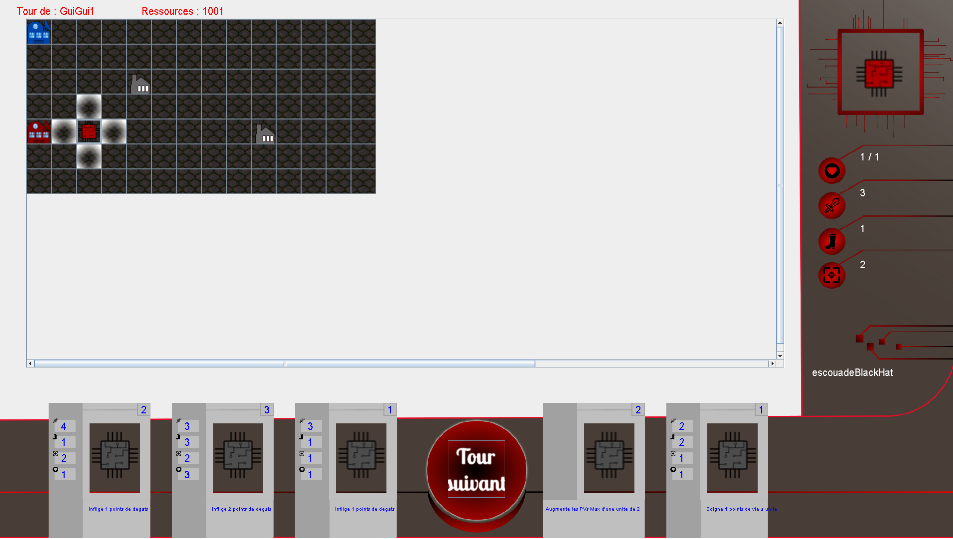
\includegraphics[scale=0.3]{Assets/UniteeSelectMove.png} 
        \end{center}

  
  \chapter{Bilan}
    \section{Bilan pédagogique}
      Ce projet nous a permit de renforcer nos acquis dans des langages tels que \textit{Java}, \textit{MySQL} ou encore \textit{PHP} avec le \textit{framework} <<silex>>. Mais ce projet nous également permit d'acquérir de nouvelle connaissance, notamment comment lié \textit{Mysql} a \textit{Java}, ou encore la communication réseaux en \textit{Java}. Ce projet, et quelques mésaventures avec des modifications de code altérant le bon fonctionnement du programme, nous a appris que la pratique du test logiciel était importante pour la programmation d'un jeu.
      
    \section{Bilan technique}
       Nous avons à l'heure actuelle un programme fonctionnel malgré quelques failles notamment dû à un manque de rigueur dans la gestion des contrôleurs, mais également de quelques problèmes avec les effets. Certains de ceux-ci ne s'appliquent pas. Si notre programme reste viable dans le fond, la forme reste encore à améliorer. En effet, toutes les cartes n'ont pas encore d'images et l'interface générale du reste minime. Les points évoqués précédemment correspondent aux potentielles voix d'améliorations du projet.

\end{document}
